\section{Evaluation}

\begin{figure}[t]  %%%%%%%%%%%%%%%%%%%%%%%
\centerline{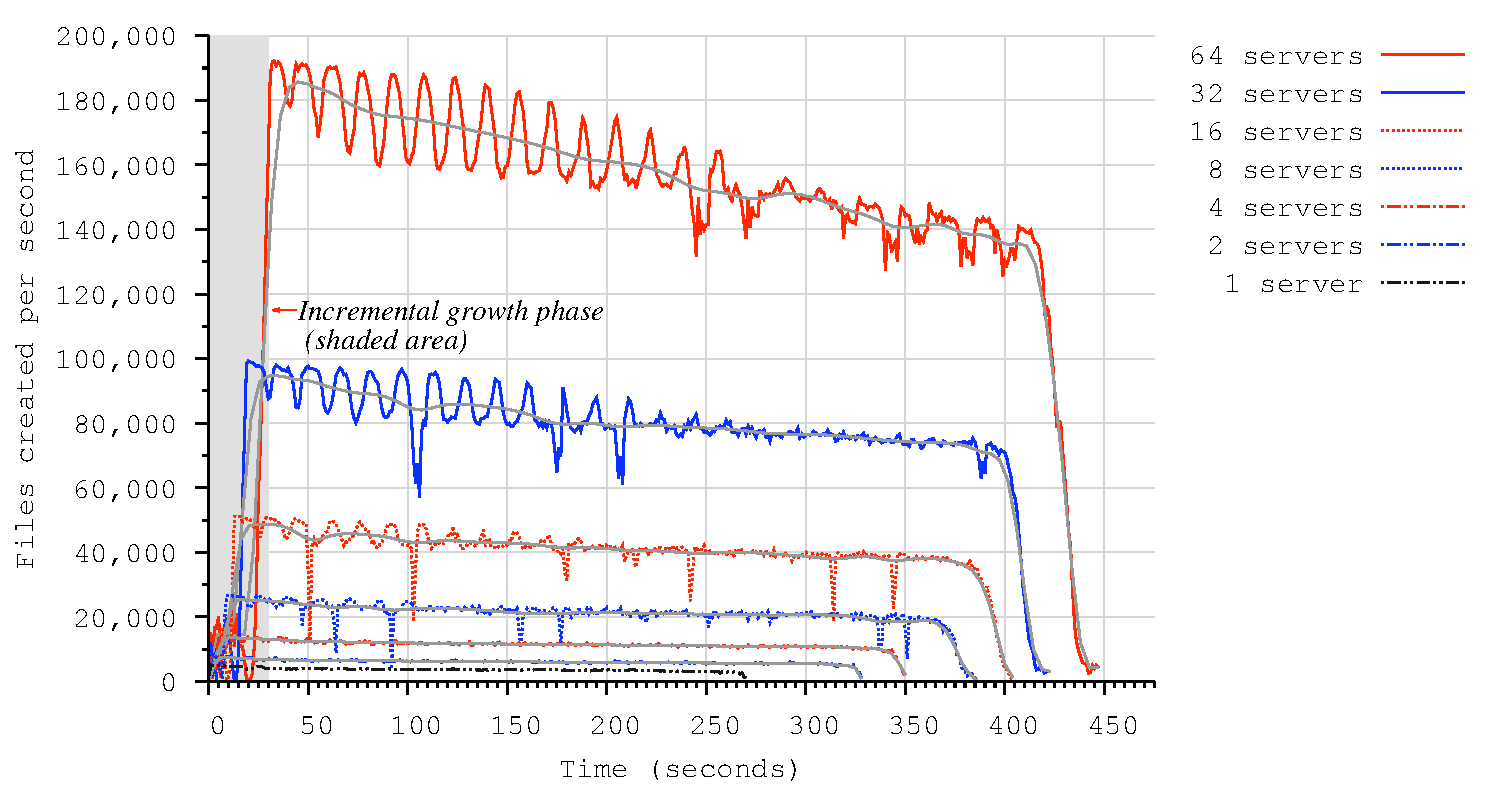
\includegraphics[scale=0.33]{./figs/ldb_insertrate}}
\caption{
\textbf{Scale-out performance on an on-disk LevelDB backend.}
{\small
\giga{} using a disk-based LevelDB backend shows promising scalability
up to 64 servers. However the interaction between LevelDB's compaction policies and 
the Linux Ext3's implementation policies causes periodic throughput variance
that degrades as the the number of directory entries in each LevelDB
increases. \textit{Note that the solid lines in each configuration are Bezier
curves to smooth the variability.}
}
}
\vspace{15pt}
\hrule 
\label{graph:ldb-scaling}
\end{figure}       %%%%%%%%%%%%%%%%%%%%%%%

Figure \ref{graph:ldb-scaling} shows the instantaneous throughput during the 
\textit{concurrent create} workload in a strong scaling experiment, i.e.
creating 1 million files per server and reaching up to 64 million files in the
64 server configuration.
The main result in this figure is that as the number of servers doubles the
throughput of the system also scales up. With 64 servers, \giga{} can achieve a
peak throughput of about 190,000 file creates per second. The system delivers
this peak performance after the directory workload has been spread among all
servers.
Before reaching steady-state, the throughput grows gradually due to the splitting
policies adopted by \giga{}. We take a closer look at this incremental growth in
the next chapter.

Another key observation in Figure \ref{graph:ldb-scaling} is that the system is
unable to sustain the steady-state peak throughput: in fact, in large setups
with 8 or more servers, the peak throughput drops by as much as 25\% (in case
of the 64-server setup). 
This happens for two reasons, both related to the policies and behavior of
LevelDB.

\begin{figure}[t]  %%%%%%%%%%%%%%%%%%%%%%%
\centerline{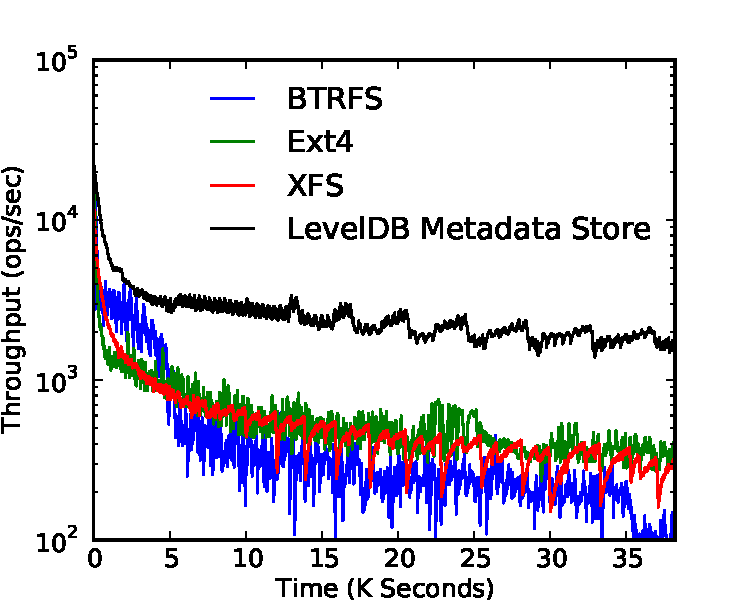
\includegraphics[scale=0.45]{./figs/ldb_insertrate_onenode}}
\caption{
\textbf{Single-node LevelDB performance compared to three Linux filesystems.}
{\small
A one-server configuration with LevelDB backend shows the performance of creating 100 million zero-length files.
We only graph the time until LevelDB finished inserting all 100 million zero-length files, 
because the other file systems were much slower. LevelDB is 10X faster than the other tested file systems.
The veritical axis is in a log scale.
}
}
\vspace{15pt}
\hrule 
\label{graph:ldb-singlenode}
\end{figure}       %%%%%%%%%%%%%%%%%%%%%%%

The first reason is periodic \textit{compactions} in LevelDB that create
ordered files 
by periodically sorting the in-memory log and writing them to separate files 
on-disk. If there are pre-existing files from previous compactions, LevelDB merges 
these old files with newly arrived in-memory logs to write out most recent sorted 
sequential files. These compactions cause both read and write disk I/O:
existing sorted files are read into memory and newly merged files are written
back to disks. Figure \ref{graph:ldb-singlenode} shows the variability in insert
throughput of a single node instance of LevelDB-based backend. This figure
shows that periodic background compactions happen during the entire experiment
which causes the throughput to drop steadily -- the overall throughput drop is
more than 35\% of the peak throughput.
In Figure \ref{graph:ldb-scaling}, the throughput drop is much higher in
aggregate but is about the same fraction as the single-node degradation.
This is expected because each LevelDB instance performs these compactions, and 
because each \giga{} server handles a uniform load, all LevelDB instances are busy
performing compactions.  

The second reason for the degrading saw-tooth behavior in Figure
\ref{graph:ldb-scaling} is due to the choice of LevelDB key used by \tfs{}.
Recall that \tfs{} uses a combination of the file name, the parent directory's
unique identifier and the hash value of the file name as the key. 
The hash value of the file name causes an interesting tradeoff: it simplifies
LevelDB's split optimizations but it makes LevelDB's compactions more I/O
intensive.
Because the hash values are uniformly random, even two lexicographically
similar file names in the same parent directory will have random, and
lexicographically very different, hash values.
This makes the entire LevelDB key lexicographically different which causes
LevelDB to read more files during compactions.

To confirm our hypothesis, we compared the variability in LevelDB's insert
throughput for different keys.
Figure "comingInTheFuture" will hopefully how this tradeoff (XXX).
%XXX: function of different keys and values 

